\chapter{Приложение}
\label{ch:appendix}

\section{Приложение А. Экспериментальная установка}
Схема экспериментальной установки изображена на Рис. 3. Поток воздуха под давлением, немного превышающим атмосферное, поступал через газовый счётчик в тонкие металлические трубки. Воздух нагнетался компрессором, интенсивность его подачи регулировалась краном К. Трубки снабжены съёмными заглушками на концах и рядом миллиметровых отверстий, к которым можно подключать микроманометр. В рабочем состоянии открыта заглушка на одной (рабочей) трубке, микроманометр подключён к двум её выводам, а все остальные отверстия плотно закрыты пробками. Перед входом в газовый счётчик установлен водяной U-образный манометр. Он служил для измерения давления газа на входе, а также предохранял счётчик от выхода из строя. При превышении максимального избыточного давления на входе счётчика ($\sim$ 30 см вод. ст.) вода выплёскивалась из трубки в защитный баллон Б, создавая шум и привлекая к себе внимание экспериментаторов.

\begin{figure}[h!]
        \centering
        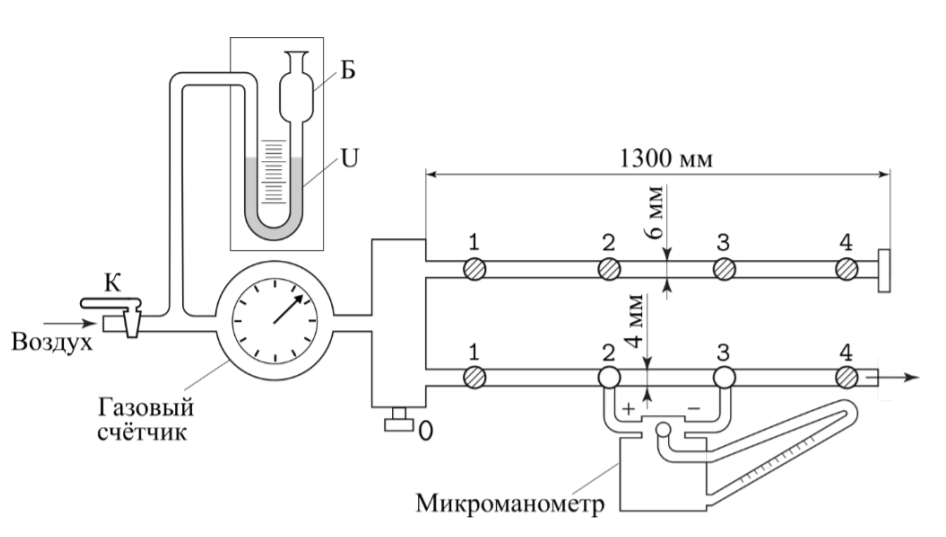
\includegraphics[scale=0.8]{img/expust.png}
        
        \centering Рис. 6. Экспериментальная установка для определения вязкости воздуха в тонких трубках. Поток воздуха под давлением, немного превышающим атмосферное, поступал через газовый счётчик в тонкие металлические трубки. Воздух нагнетался компрессором, интенсивность его подачи регулировалась краном К. Трубки снабжены съёмными заглушками на концах и рядом миллиметровых отверстий, к которым можно подключать микроманометр. В рабочем состоянии открыта заглушка на одной (рабочей) трубке, микроманометр подключён к двум её выводам, а все остальные отверстия плотно закрыты пробками. Перед входом в газовый счётчик установлен водяной U-образный манометр. Он служил для измерения давления газа на входе, а также предохранял счётчик от выхода из строя. При превышении максимального избыточного давления на входе счётчика ($\sim$ 30 см вод. ст.) вода выплёскивалась из трубки в защитный баллон Б, создавая шум и привлекая к себе внимание экспериментаторов.
 \end{figure} 
\vspace{10pt}
Приборы и данные:
\begin{itemize}
    \item Термогигрометр с функцией отображения давления $testo \ 622$, погрешность измерения давления 3 гПа, температуры - 0,4 $^\circ C$, влажности - 2\% в диапазоне от 0 до 90 \%
    \item Микроманометр ММН-2400(5)-1б0, погрешность при различных K: 6 Па ($K = 0,2$), 9 Па ($K = 0,3$), 12 Па ($K = 0,4$), 18 Па ($K = 0,6$).
    \item Счетчик газовый барабанный модель ВИКС-1, погрешность измерения 1\%
\end{itemize}
\newpage

\section{Приложение Б. Результаты измерений}

\begin{table}[h]
\begin{tabular}{|c|c|c|}
\hline
{$\Delta P$, дел} & {$\Delta P$, Па} & {$Q$, л/мин} \\
\hline
10 & 19.61 & 0.6 \\ \hline
20 & 39.23 & 1.4 \\ \hline
30 & 58.84 & 2.1 \\ \hline
40 & 78.45 & 2.8 \\ \hline
50 & 98.07 & 3.6 \\ \hline
60 & 117.68 & 4.2 \\ \hline
70 & 137.29 & 4.9 \\ \hline
76 & 149.06 & 5.3 \\ \hline
80 & 156.91 & 5.4 \\ \hline
90 & 176.52 & 5.7 \\ \hline
100 & 196.13 & 5.8 \\ \hline
110 & 215.75 & 6 \\ \hline
120 & 235.36 & 6.2 \\ \hline
150 & 294.20 & 6.8 \\ \hline
200 & 392.27 & 7.7 \\ \hline
240 & 470.72 & 8.4 \\ \hline
\end{tabular}
\caption{
\centering Зависимость расхода $Q$ от перепада давления $\Delta P$ для трубки диаметром d = 3.95 мм. 
}
\end{table}

\begin{table}[h]
\begin{tabular}{|c|c|c|}
 \hline
{$\Delta P$, дел} & {$\Delta P$, Па} & {$Q$, л/мин} \\
 \hline
4 & 7.85 & 0.7 \\  \hline
8 & 15.69 & 1.6 \\ \hline
12 & 23.54 & 2.7 \\ \hline
16 & 31.38 & 3.4 \\ \hline
20 & 39.23 & 4.4 \\ \hline
24 & 47.07 & 5.3 \\ \hline
28 & 54.92 & 6 \\ \hline
32 & 62.76 & 6.7 \\ \hline
40 & 78.45 & 7.6 \\ \hline
80 & 156.91 & 10.1 \\ \hline
100 & 196.13 & 11.4 \\ \hline
120 & 235.36 & 12.7 \\ \hline
140 & 274.59 & 13.7 \\ \hline
160 & 313.81 & 14.9 \\ \hline
170 & 333.43 & 16.0 \\ \hline
\end{tabular}
\caption{
\centering Зависимость расхода $Q$ от перепада давления $\Delta P$ для трубки диаметром d = 5.05 мм. 
}
\end{table}